\documentclass{beamer}
\usepackage[utf8]{inputenc}

\usetheme{Boadilla}
\usecolortheme{lily}
\usepackage{amsmath,amssymb,amsfonts,amsthm}
\usepackage{mathtools}
\usepackage{txfonts}
\usepackage{tkz-euclide}
\usepackage{listings}
\usepackage{adjustbox}
\usepackage{array}
\usepackage{tabularx}
\usepackage{lmodern}
\usepackage{gvv}
\usepackage{circuitikz}
\usepackage{tikz}
\usepackage{graphicx}

\setbeamertemplate{footline}
{
  \leavevmode%
  \hbox{%
  \begin{beamercolorbox}[wd=\paperwidth,ht=2.25ex,dp=1ex,right]{author in head/foot}%
    \insertframenumber{} / \inserttotalframenumber\hspace*{2ex} 
  \end{beamercolorbox}}%
  \vskip0pt%
}

\usepackage{tcolorbox}
\tcbuselibrary{minted,breakable,xparse,skins}




\providecommand{\nCr}[2]{\,^{#1}C_{#2}} % nCr
\providecommand{\nPr}[2]{\,^{#1}P_{#2}} % nPr
\providecommand{\mbf}{\mathbf}
\providecommand{\pr}[1]{\ensuremath{\Pr\left(#1\right)}}
\providecommand{\qfunc}[1]{\ensuremath{Q\left(#1\right)}}
\providecommand{\sbrak}[1]{\ensuremath{{}\left[#1\right]}}
\providecommand{\lsbrak}[1]{\ensuremath{{}\left[#1\right.}}
\providecommand{\rsbrak}[1]{\ensuremath{{}\left.#1\right]}}
\providecommand{\brak}[1]{\ensuremath{\left(#1\right)}}
\providecommand{\lbrak}[1]{\ensuremath{\left(#1\right.}}
\providecommand{\rbrak}[1]{\ensuremath{\left.#1\right)}}
\providecommand{\cbrak}[1]{\ensuremath{\left\{#1\right\}}}
\providecommand{\lcbrak}[1]{\ensuremath{\left\{#1\right.}}
\providecommand{\rcbrak}[1]{\ensuremath{\left.#1\right\}}}
\theoremstyle{remark}
\newcommand{\sgn}{\mathop{\mathrm{sgn}}}
\providecommand{\abs}[1]{\left\vert#1\right\vert}
\providecommand{\res}[1]{\Res\displaylimits_{#1}} 
\providecommand{\norm}[1]{\lVert#1\rVert}
\providecommand{\mtx}[1]{\mathbf{#1}}
\providecommand{\mean}[1]{E\left[ #1 \right]}
\providecommand{\fourier}{\overset{\mathcal{F}}{ \rightleftharpoons}}
%\providecommand{\hilbert}{\overset{\mathcal{H}}{ \rightleftharpoons}}
\providecommand{\system}{\overset{\mathcal{H}}{ \longleftrightarrow}}
	%\newcommand{\solution}[2]{\textbf{Solution:}{#1}}
%\newcommand{\solution}{\noindent \textbf{Solution: }}
\providecommand{\dec}[2]{\ensuremath{\overset{#1}{\underset{#2}{\gtrless}}}}
\newcommand{\myvec}[1]{\ensuremath{\begin{pmatrix}#1\end{pmatrix}}}
\let\vec\mathbf

\lstset{
%language=C,
frame=single, 
breaklines=true,
columns=fullflexible
}

\numberwithin{equation}{section}

\lstset{
  language=Python,
  basicstyle=\ttfamily\small,
  keywordstyle=\color{blue},
  stringstyle=\color{orange},
  numbers=left,
  numberstyle=\tiny\color{gray},
  breaklines=true,
  showstringspaces=false
}

\title{Problem 10.3.26}
\author{ee25btech11023-Venkata Sai}

\date{\today} 
\begin{document}

\begin{frame}
\titlepage
\end{frame}

\section*{Outline}
\begin{frame}
\tableofcontents
\end{frame}

\section{Problem}

\begin{frame}
\frametitle{Problem}
Find the point at which the tangent to the curve $y = \sqrt{4x-3}-1$ has its slope $\frac{2}{3}$ 
\end{frame}
%\subsection{Literature}
\section{Solution}

 
\subsection{Equation}
\begin{frame}
\frametitle{Equation}
Given curve
\begin{align}
y &= \sqrt{4x-3}-1 \\
y+1=\sqrt{4x-3} &\implies \brak{y+1}^2 =4x-3 \\
y^2&+2y+1=4x-3 \\
y^2&-4x+2y+4=0
\end{align}
Equation \brak{4} in matrix form
\begin{align}
y^2+2\brak{-2x+y}+4=0 \\
\vec{x}^\top\myvec{0&0\\0&1}\vec{x}+2\myvec{-2&1}\vec{x}+4=0
\end{align}
The general equation of conic
\begin{align}
    \vec{x}^\top\vec{V}\vec{x} + 2\vec{u}^\top\vec{x} + f = 0
\end{align}
On comparing \brak{6} with \brak{7}

\end{frame}
\subsection{Simplify}
\begin{frame}
\frametitle{Simplify}
\begin{align}
\vec{V}=\myvec{0&0\\0&1},\vec{u}=\myvec{-2\\1},f=4
\end{align}
Given slope
\begin{align}
    m=\frac{2}{3}
\end{align}
The normal vector to the given tangent is 
\begin{align}
    \vec{n}=\myvec{-m\\1} \implies \vec{n}=\myvec{-\frac{2}{3}\\1} 
    \end{align}
    \begin{align}
    |\vec{V}-& \lambda\vec{I}|=0 \\
    \mydet{\myvec{0&0\\0&1}-\lambda\myvec{1&0\\0&1}}=0 &\implies
    \mydet{\myvec{0&0\\0&1}-\myvec{\lambda&0\\0&\lambda}}=0\\
    \mydet{\myvec{-\lambda&0\\0&1-\lambda}}=0 &\implies \brak{-\lambda}\brak{1-\lambda}=0 \\
    \lambda_1=0\ &\text{and}\ \lambda_2=1
\end{align}
 \end{frame}
 \subsection{Finding the variables}
\begin{frame}
\frametitle{Finding the variables}
Finding eigen vector for $\lambda_1=0$
\begin{align}
    \brak{\vec{V}- \lambda\vec{I}}\vec{p}&=\vec{0}\\
    \myvec{-\lambda&0\\0&1-\lambda}\myvec{x\\y}=0 &\implies \myvec{0&0\\0&1}\myvec{x\\y}=\myvec{0\\0}\\
     0=0,y=0 &\implies \vec{p_1}=\myvec{1\\0}
\end{align}
For a given normal vector $\vec{n}$, the point of contact $\vec{q}$ for a given curve is given by the matrix equation
\begin{align}
\myvec{\brak{\vec{u}+\kappa\vec{n}}^\top\\\vec{V}}\vec{q}=\myvec{-f\\\kappa\vec{n}-\vec{u}} \quad\ &\text{where}\ \kappa=\frac{\vec{p_1}^\top\vec{u}}{\vec{p_1}^\top\vec{n}} \\
\kappa=\frac{\myvec{1&0}\myvec{-2\\1}}{\myvec{1&0}\myvec{-\frac{2}{3}\\1}}&=\frac{-2}{-\frac{2}{3}}=3
\end{align}
 \end{frame}
\begin{frame}
\subsection{Conclusion}
\frametitle{Conclusion}
 From \brak{8}
 \begin{align}
\myvec{\brak{\myvec{-2\\1}+3\myvec{-\frac{2}{3}\\1}}^\top\\\myvec{0&0\\0&1}}&\vec{q}=\myvec{-4\\3\myvec{-\frac{2}{3}\\1}-\myvec{-2\\1}} \\
\myvec{\myvec{-4\\4}^\top\\\myvec{0&0\\0&1}}\vec{q}=\myvec{-4\\\myvec{-2\\3}+\myvec{2\\-1}} &\implies 
\myvec{\myvec{-4&4}\\\myvec{0&0\\0&1}}\vec{q}=\myvec{-4\\\myvec{0\\2}}
\end{align}
\begin{align}
\myvec{-4&4\\0&0\\0&1}\vec{q}&=\myvec{-4\\0\\2} 
\end{align}
\end{frame}
\begin{frame}
\frametitle{Conclusion}
Taking augmented matrix
\begin{align}
    \augvec{2}{1}{-4&4&-4\\0&0&0\\0&1&2}\xrightarrow{R_1\rightarrow R_1-4R_2}\augvec{2}{1}{-4&0&-12\\0&0&0\\0&1&2}\xrightarrow{R_1\rightarrow-\frac{1}{4}R_1}\augvec{2}{1}{1&0&3\\0&0&0\\0&1&2} 
    \end{align}
    \begin{align}
    \vec{q}=\myvec{3\\2}
\end{align}
 Hence the point of contact is $\myvec{3\\2}$
\end{frame}
\subsection{Plot}
\begin{frame}[fragile]
\frametitle{Plot}

\begin{figure}[h!]
   \centering
   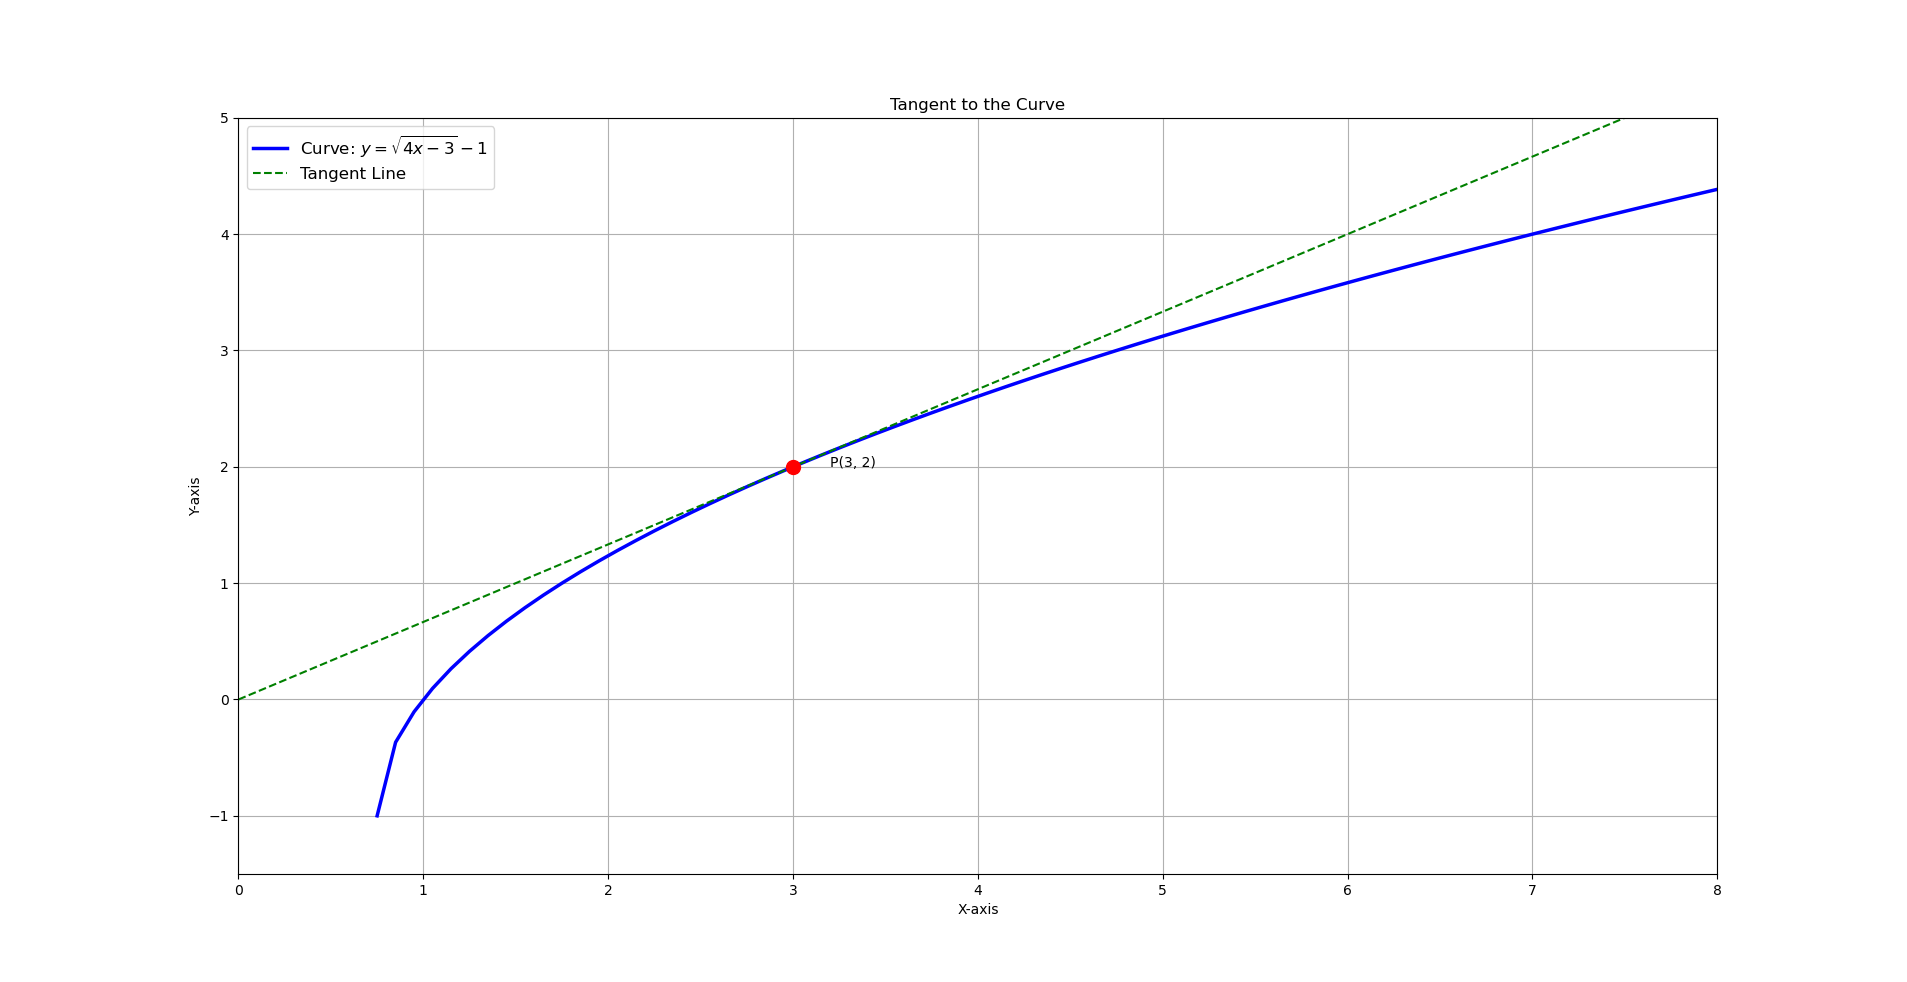
\includegraphics[width=0.9\columnwidth]{figs/fig1.png}
	\caption{}
   \label{}
\end{figure}
\end{frame}

\section{C Code}
\begin{frame}[fragile]
\frametitle{C Code}
\begin{lstlisting}[language=C]
#include <math.h>

void get_tangent_data(double* out_data) {
       double tangent_x = 3.0;
    double tangent_y = 2.0;
        int num_points = 101;
    out_data[0] = tangent_x;
    out_data[1] = tangent_y;

    int index = 2;
    for (int i = 0; i < num_points; i++) {
        double x = 0.75 + (10.0 * i) / (num_points - 1);

        out_data[index]     = x;
        out_data[index + 1] = sqrt(4 * x - 3) - 1;
        index += 2;
    }
}


    \end{lstlisting}
\end{frame}

\section{Python Code}
\begin{frame}[fragile]
\frametitle{Python Code for Solving}
\begin{lstlisting}[language=Python]
import ctypes
import numpy as np

def get_data_from_c():
    lib = ctypes.CDLL('./code.so')
    data_size = 2 + (101 * 2)
    double_array = ctypes.c_double * data_size
    lib.get_tangent_data.argtypes = [ctypes.POINTER(ctypes.c_double)]

    out_data_c = double_array()
    lib.get_tangent_data(out_data_c)

    all_data = np.array(out_data_c)
    tangent_point = all_data[0:2]
    curve_points = all_data[2:].reshape((-1, 2))
    return tangent_point, curve_points



\end{lstlisting}
\end{frame}
 
\begin{frame}[fragile]
\frametitle{Python Code for Plotting}
\begin{lstlisting}[language=Python]
# Code by /sdcard/github/matgeo/codes/CoordGeoVV Sharma
# September 12, 2023
# Revised July 21, 2024
# Released under GNU GPL
# Section Formula
import sys
sys.path.insert(0, '/workspaces/urban-potato/matgeo/codes/CoordGeo/') 
import numpy as np
import matplotlib.pyplot as plt

from call import get_data_from_c
P, curve_points = get_data_from_c()
slope = 2.0 / 3.0
x_tangent = np.array([0, 8])
y_tangent = slope * (x_tangent - P[0]) + P[1]
fig, ax = plt.subplots(figsize=(10, 8))
ax.plot(curve_points[:, 0], curve_points[:, 1], 'b-', linewidth=2.5, label='Curve: $y = \\sqrt{4x-3} - 1$')

\end{lstlisting}
\end{frame}
\begin{frame}[fragile]
\frametitle{Python Code for Plotting}
\begin{lstlisting}[language=Python]
ax.plot(x_tangent, y_tangent, 'g--', label='Tangent Line')

ax.scatter(P[0], P[1], color='red', s=100, zorder=5)
ax.text(P[0] + 0.2, P[1] + 0.2, f'P({P[0]:.0f}, {P[1]:.0f})')

ax.set_title('Tangent to the Curve')
ax.set_xlabel('X-axis')
ax.set_ylabel('Y-axis')
ax.set_xlim(0, 8)
ax.set_ylim(-1.5, 5)

ax.grid(True)
ax.legend(fontsize=12)

plt.show()
plt.savefig('fig.png')
           
\end{lstlisting}
\end{frame}
 
\end{document}
